\documentclass{standalone}
\usepackage{pgfplots}
\pgfplotsset{compat=1.18}

\begin{document}
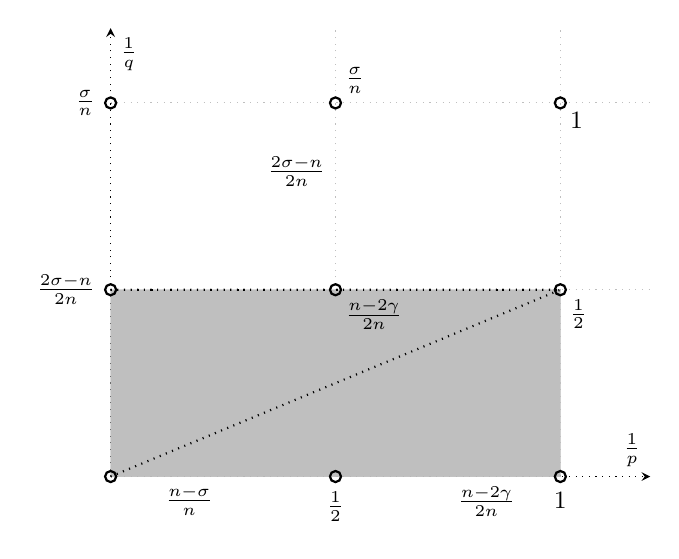
\begin{tikzpicture}
    \begin{axis}[
        axis lines=middle,
        xlabel=$\frac{1}{p}$,
        ylabel=$\frac{1}{q}$,
        xmin=0, xmax=1.2,
        ymin=0, ymax=1.2,
        xtick={0, 0.5, 1},
        ytick={0, 0.5, 1},
        xticklabels={$O$, $\frac{1}{2}$, $1$},
        yticklabels={$\frac{2\sigma-2\gamma-n}{2n}$, $\frac{2\sigma-n}{2n}$, $\frac{\sigma}{n}$, $\frac{1}{2}$, $1$},
        grid=major,
        dotted,
        clip=false,
        every axis plot/.append style={thick},
        every tick label/.append style={font=\small},
        every axis/.append style={font=\small},
    ]
        
        % Plot the shaded region
        \addplot[fill=gray!50, draw=none, domain=0:1] {1/2} \closedcycle;
        \addplot[fill=gray!50, draw=none, domain=0:1] {x/2} \closedcycle;
        \addplot[fill=gray!50, draw=none, domain=0:1] {x/2 + (1-x)/2} \closedcycle;
        
        % Plot the boundary lines
        \addplot[domain=0:1, samples=100] {1/2};
        \addplot[domain=0:1, samples=100] {x/2};
        \addplot[domain=0:1, samples=100] {x/2 + (1-x)/2};
        
        % Mark points
        \addplot[only marks, mark=o, mark options={solid}] coordinates {(0,0) (0.5,0) (1,0)};
        \addplot[only marks, mark=o, mark options={solid}] coordinates {(0,0.5) (0.5,0.5) (1,0.5)};
        \addplot[only marks, mark=o, mark options={solid}] coordinates {(0,1) (0.5,1) (1,1)};
        
        % Annotations
        \node at (axis cs:0.5,0.5) [below right] {$\frac{n-2\gamma}{2n}$};
        \node at (axis cs:0.5,0.75) [above left] {$\frac{2\sigma-n}{2n}$};
        \node at (axis cs:0.5,1) [above right] {$\frac{\sigma}{n}$};
        \node at (axis cs:0.25,0) [below left] {$\frac{n-\sigma}{n}$};
        \node at (axis cs:0.75,0) [below right] {$\frac{n-2\gamma}{2n}$};
        \node at (axis cs:1,0.5) [below right] {$\frac{1}{2}$};
        \node at (axis cs:1,1) [below right] {$1$};
        
    \end{axis}
\end{tikzpicture}
\end{document}